\section{IMPLICIT DOMAIN-SPECIFIC RECOMMENDATION MODELS}
In this section, the IDSR model is elaborated in detail. In general, it consists of four parts.(see figure 2)
\begin{figure}[h]
	\caption{The framework of IDSR}
	\centering
	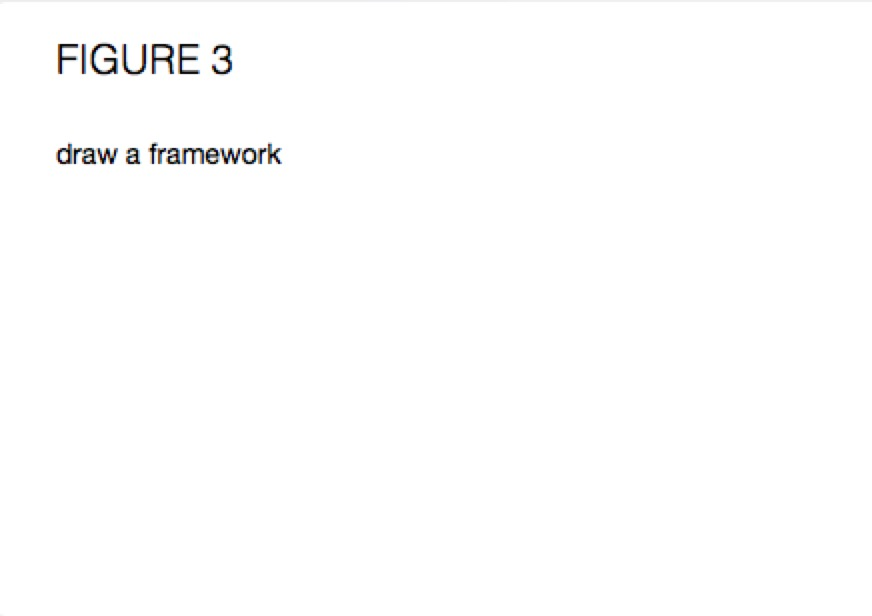
\includegraphics[width=8cm]{framework}
\end{figure}
Firstly, the items are clustered into small groups, which is defined as \emph{domains}, according to their content information such as titles and tags of movies in MovieLens dataset. Then, based on an assumption that users will trust those who share similar interest with them in specific domains, the domain-specific trust network is constructed with several trust assignment methods. Further, the rating matrix is split into domain-specific trust-based sub matrices. Finally, the model is trained by gradient descent methods.
\subsection{Implicit Domain Inference}
The sparsity and cold start are the two main challenges facing the current recommendation algorithms. To address these two problems, many researchers started to employ side information such as social connections between users and text information of items. Examples of former one are the aforementioned social- or trust-based recommendation systems while the latter ones always occur in content-based recommendation system.

In this work, the text information of items are utilized to cluster the items into small groups, namely domains. We choose the popular latent dirichlet allocation (LDA)\cite{blei2003latent} as my clustering model, which is useful methods to extract hidden topics, i.e. domains, from rich text information. By tuning the parameters, a specific number of topics are learned from the texts of items. Then we get the domains needed to split the trust network between users.

\textcolor{red}{\textbf{give examples about topics in Movielens and amazon data}}
\textcolor{red}{\textbf{better to draw some pictures}}

\textcolor{red}{\textbf{better to use more math symbols than text descriptions}}

\subsection{Domain-Specific trust Network}
Given the domains of items learned by LDA, we then construct the domain-specific trust network between users.The basic idea is that a user may only trust those who are similar to him/her in the specific domains. For example, the trust people concerning the Spielberg's Movies can differ significantly from those regarding romantic movies.

Therefore, we split the network $S$ of all implicit trust relationships inferred before into many domain-specific sub-networks $S^{(d)}$, each of which concerning a single domain $d$ of items. Very similar to the definition in \cite{yang2012circle}, we also give the domain-specific trust networks of users in the following.

\textbf{Definition(Domain-Specific Trust network)}: \emph{Regarding each domain $d$, users $u$ and $v$ are not in the same sub-network of trust between them, if and only if the following two criterions are satisfied:
	\begin{itemize}
		\item $T_{u,v} > 0$ in the inferred trust network, and
		\item $N_u^{(d)} > 0$ and $N_v^{(d)} > 0$ in the rating data, 
	\end{itemize}
where $N_u^{(d)}$ denotes the number of rating that user $u$ has assigned to items in domain $d$. Otherwise $u$ and $v$ are not in the trust network regarding domain d, which means they have no trust relations between each other concerning domain $d$, i.e. $v \notin T_u^{d}$.
	}

This is illustrated for a toy example in Figure 3.
\begin{figure}[h]
	\caption{Toy Example for trust network concerning different domains}
	\centering
	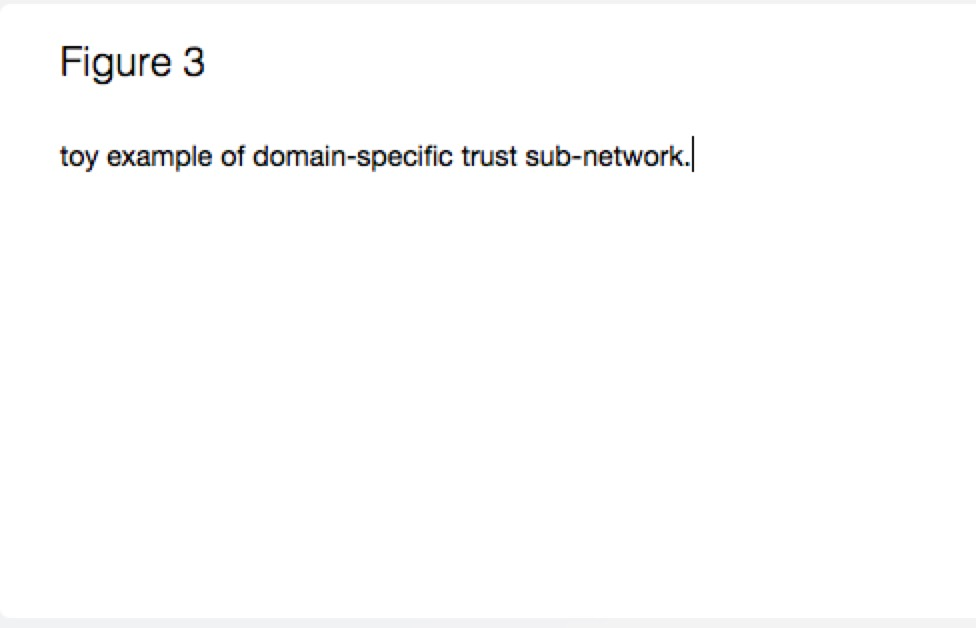
\includegraphics[width=8cm]{toy_example}
\end{figure}

\textcolor{red}{\textbf{The definition need to be adjusted, draw some pictures like the circle-based paper and must modify the elaboration in the beginning of this section}}

\subsection{Trust Assignment}
After we construct the domain-specific trust network, we need to infer the trust of a user $u$ in a user $v$ regrading one specific domain. The whole process is based on one assumption that \emph{we trust people who share the same preferences over items in corresponding domains.} And the similarity is computed by the popular Pearson Correlation Coefficient (PCC)\cite{breese1998empirical}, which is used to define the similarity between two users $u$ and $v$ based on the items they rated in common:
\begin{equation}
Sim(u, v) = \frac{\sum\limits_{j \in I(u) \cap I(v) }R_{uj} \centerdot R_{vj}}{\sqrt{\sum\limits_{j \in I(u) \cap I(v)}R_{uj}^2} \centerdot \sqrt{\sum\limits_{j \in I(u) \cap I(v)}R_{vj}^2}},
\end{equation}
This formula takes the whole rating matrix into consideration. Therefore, in our domain-specific trust inferring algorithm, the similarity between two users $u$ and $v$ regarding the domain $d$ should be written as follows:
\begin{equation}
Sim^{(d)}(u, v) = \frac{\sum\limits_{j \in I^{(d)}(u) \cap I^{(d)}(v) }R_{uj} \centerdot R_{vj}}{\sqrt{\sum\limits_{j \in I^{(d)}(u) \cap I^{(d)}(v)}R_{uj}^2} \centerdot \sqrt{\sum\limits_{j \in I^{(d)}(u) \cap I^{(d)}(v)}R_{vj}^2}},
\end{equation}

Then we use a very heuristic method that maps the similarity to trust value, in which we just assign the similarity value to the trust.
\textcolor{red}{\textbf{assumption: similar users generate trust
		domain-specific similarity 
		pcc metric
		trust assignment  $\rightarrow$ similar to circle-based}}

\subsection{Model Training}
According to two regularization methods in \cite{ma2011recommender}, we use the trust set users $T_u^{(d)}$of one user in a specific domain $d$ as regularization terms to integrate into the MF framework and we adopt the individual-based regularization method. The only difference is that we train the model for different domains.
For a domain $d$, the training objective function is as follows:
\begin{equation}
\begin{aligned}
\mathcal{L}^{(d)}(R^{(d)}, U^{(d)}, V^{(d)}, S^{(d)}) &= \frac{1}{2}\sum_{i=1}^{m}\sum_{j=1}^{n}I^{(d)}_{ij}(R^{(d)}_{ij} - {U_i^{(d)}}^TV^{(d)}_j)^2 + \frac{\beta}{2}\sum_{i=1}^{m}\sum_{f \in \phi^{(d)}(U_i)}Sim(U^{(d)}_i, U^{(d)}_f)||U^{(d)}_i - U^{(d)}_f||_F^2
\\ 
&+ \frac{\lambda_1}{2}||U^{(d)}||_F^2 + \frac{\lambda_2}{2}||V^{(d)}||_F^2,
\end{aligned}
\end{equation}
where $\phi^{(d)}(U_i)$ is the trust set of the user $U_i$ regarding domain $d$. In the experiment, we choose top k of the trust set of user $U_i$ where k is a parameter that can be tuned.

Analogous to \cite{ma2011recommender} and \cite{yang2012circle}, the gradient descent approach is exploited to minimize the Equation (14). 
\begin{equation}
\begin{aligned}
\frac{d\mathcal{L}^{(d)}}{dU_i^{(d)}} &= \sum_{j=1}^{n}I^{(d)}_{ij}({U_i^{(d)}}^TV^{(d)}_j - R^{(d)}_{ij})V^{(d)}_j+\beta\sum_{f \in \phi^{(d)}(U_i)}Sim(U^{(d)}_i, U^{(d)}_f)(U^{(d)}_i - U^{(d)}_f) + \lambda_1 U_i^{(d)},
\\
\frac{d\mathcal{L}^{(d)}}{dV_i^{(d)}} &= \sum_{i=1}^{m}I^{(d)}_{ij}({U_i^{(d)}}^TV^{(d)}_j - R^{(d)}_{ij})U^{(d)}_j + \lambda_2 V_i^{(d)},
\end{aligned}
\end{equation}

\textcolor{red}{\textbf{double-check the correctness of the formulas}}
\textcolor{red}{\textbf{introduce every variables regarding the dimensions and meanings.}}

\subsection{Complexity Analysis}
The computational cost of the model lies in mainly three aspects: clustering, evaluation of the objective function $\mathcal{L}$ and its gradients with respect to variables. Firstly, the clustering can be done offline, thus its computation cost can be regarded as constant. And speaking of the latter two aspects, due to the sparsity of matrices R and T, the complexity of evaluating the objective function $\mathcal{L}$ is $O(l|\Omega| + lmk|D|)$, where l is the dimension of user\-specific latent vector, $|\Omega|$ is the number of ratings in the original rating matrix, $m$ is the number of users, $|D|$ is the number of the domains, which can be defined when running the LDA model, and $k$ is the average number of trust people of one user in one domain. On the other hand, the complexity of evaluating the gradients with respect to $U$ and $V$ is  $O(l|\Omega| + lmk|D|)$ and $O(l|\Omega|)$, respectively. Therefore, the total computational complexity in one iteration is $O(l|\Omega| + lmk|D|)$, which indicates that the computational time of my model is linear with respect to the number of the observations in the rating and trust matrices, which are very sparse in reality. This complexity analysis shows that the proposed approach is very efficient and can scale to very large datasets.




